\chapter{Mohr-Coulomb model}

\section{Introduction}
The classical Mohr-Coulomb model is a workhorse of rock and soil plasticity modeling.
This model is typically hard to implement for implicit codes because of the
difficulties encountered in computing tangent stiffness matrices near the corners (as viewed from the
hydrostatic axis).  However, that problem is not encountered in explicit codes and corners can be
handled relatively easily.  The \Vaango implementation of Mohr-Coulomb plasticity includes two variations
on the shape of the yield surface:
\begin{itemize}
 \item the classical model
 \item the Sheng et al. variation of the yield surface~\cite{Sheng2000}.
\end{itemize}
\begin{NoteBox}
  The convention used for this model is that stresses are positive in compression and that the principal
  stresses are in the order $\sigma_1 > \sigma_2 > \sigma_3$.  The model assumes that the plastic potential
  (alternatively referred to as the dilation model) and yield function have the same form but the angles
  may differ.  The angle of the plastic potential function is denoted $\psi$.
\end{NoteBox}

\subsection{Classical Mohr-Coulomb yield surface}
The classical Mohr-Coulomb yield surface expressed in terms of the principal stresses
is
\Beq \label{eq:MC_principal}
  \Bal
  \pm\frac{\sigma_1 - \sigma_2}{2} & = \left[\frac{\sigma_1 + \sigma_2}{2}\right]\sin(\phi) + c\cos(\phi) \\
  \pm\frac{\sigma_2 - \sigma_3}{2} & = \left[\frac{\sigma_2 + \sigma_3}{2}\right]\sin(\phi) + c\cos(\phi)\\
  \pm\frac{\sigma_1 - \sigma_3}{2} & = \left[\frac{\sigma_1 + \sigma_3}{2}\right]\sin(\phi) + c\cos(\phi).
  \Eal
\Eeq
where $c$ is the cohesive strength and $\phi$ is the angle of internal friction.

The eigenvalues of the stress tensor can be computed in closed form.  The resulting expressions
are
\Beq \label{eq:stress_eig}
  %\sigma_1 = \cfrac{1}{\sqrt{3}}~\xi + \sqrt{\cfrac{2}{3}}~\rho~\cos\theta \quad \Tand \quad
  %\sigma_3 = \cfrac{1}{\sqrt{3}}~\xi + \sqrt{\cfrac{2}{3}}~\rho~\cos\left(\theta+\cfrac{2\pi}{3}\right) 
  \sigma_1 = p + \cfrac{2}{3}~q~\cos\theta \quad \Tand \quad
  \sigma_3 = p + \cfrac{2}{3}~q~\cos\left(\theta+\cfrac{2\pi}{3}\right) 
\Eeq
where
\Beq
  p = \frac{1}{3} I_1~,~~ q = \sqrt{3 J_2}~,~~
  \cos3\theta = \left(\cfrac{r}{q}\right)^3 = \frac{3\sqrt{3}}{2} \frac{J_3}{J_2^{3/2}} ~,~~
  r^3 = \frac{27}{2} J_3
\Eeq
and
\Beq
  I_1 = \Tr(\Bsig),~~ J_2 = \frac{1}{2} \Bs:\Bs,~~ J_3 = \det(\Bs),~~ \Bs = \Bsig - \frac{I_1}{3} \BI \,.
\Eeq
\begin{SummaryBox}[label=box:MC_invariant]{Classical Mohr-Coulomb yield function in terms of invariants}
In terms of these invariants, the Mohr-Coulomb yield function in \eqref{eq:MC_principal} can be expressed as
\Beq \label{eq:MC_invariant}
  f(\Bsig) = R(\theta)\,q - p~\sin\phi - c\cos\phi  
\Eeq
where 
\Beq \label{eq:R_theta}
  R(\theta) = \cfrac{1}{\sqrt{3}}~\sin\left(\theta+\cfrac{\pi}{3}\right) - 
              \cfrac{1}{3}\sin\phi~\cos\left(\theta+\cfrac{\pi}{3}\right) \,.
\Eeq
\end{SummaryBox}
Plots of the Mohr-Coulomb surface in the octahedral and Rendulic planes are shown in Figure~\ref{fig:MC}.
\begin{figure}[htbp!]
  \begin{subfigure}[t]{0.5\textwidth}
    \centering
    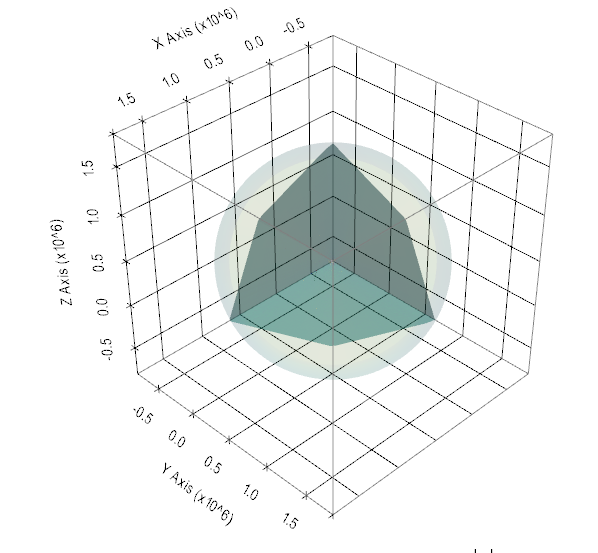
\includegraphics[width=0.9\textwidth]{Figs/mohr_coulomb/MC_octahedral_profile.png}
    \caption{Octahedral profile.}
  \end{subfigure}
  \begin{subfigure}[t]{0.5\textwidth}
    \centering
    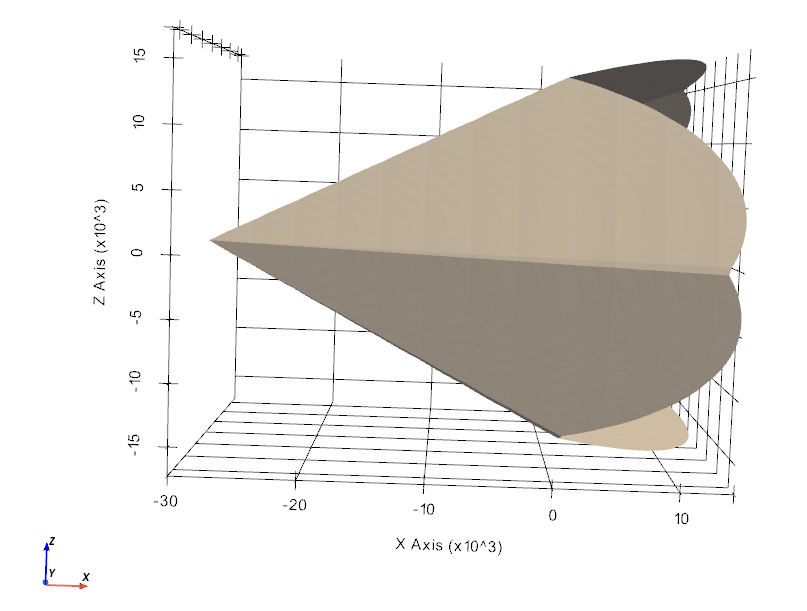
\includegraphics[width=0.9\textwidth]{Figs/mohr_coulomb/MC_rendulic.png}
    \caption{Rendulic profile.}
  \end{subfigure}
  \caption{Profiles of the classical Mohr-Coulomb yield surface.}
  \label{fig:MC}
\end{figure}

The normal to the yield surface is given by
\Beq
  \BnT = \Partial{f}{\Bsig}  = \Deriv{R}{\theta}\Partial{\theta}{\Bsig} \,q 
                              + R(\theta)\, \Partial{q}{\Bsig} 
                              - \Partial{p}{\Bsig}~\sin\phi \,.
\Eeq
where
\Beq
  \Bal
  \Deriv{R}{\theta} & = \tfrac{1}{\sqrt{3}}~\cos\left(\theta+\cfrac{\pi}{3}\right) +
                      \tfrac{1}{3}\sin\phi~\sin\left(\theta+\cfrac{\pi}{3}\right)  \\
  \Partial{\theta}{\Bsig} & = 
     -\frac{1}{\sin 3\theta}\left[\frac{9}{2 q^3} \Partial{J_3}{\Bsig} - \frac{r^3}{q^4} \Partial{q}{\Bsig}\right]
   = -\frac{1}{\sin 3\theta}\left[\frac{9}{2 q^3} \left(\Bs \cdot \Bs - \tfrac{2}{3} J_2 \BI\right) - \frac{r^3}{q^4} \Partial{q}{\Bsig} \right] \\
  \Partial{q}{\Bsig} & = \frac{\sqrt{3}}{2\sqrt{J_2}} \Partial{J_2}{\Bsig}
                     = \frac{\sqrt{3}}{2\sqrt{J_2}} \Bs  \\
  \Partial{p}{\Bsig} & = \tfrac{1}{3} \Partial{I_1}{\Bsig} = \tfrac{1}{3} \BI \,.
  \Eal
\Eeq

\subsection{Sheng et al. yield surface}
The yield function of the Mohr-Coulomb yield surface can be expressed in $p$--$q$ space as
\Beq \label{eq:Sheng}
  f(\Bsig) = q - M p - \tilde{c} \,.
\Eeq
Comparison with \eqref{eq:MC_invariant},
\Beq 
  f(\Bsig) = R(\theta)\,q - p~\sin\phi - c\cos\phi  
\Eeq
indicates that
\Beq 
  M(\theta) = \frac{\sin\phi}{R(\theta)} \quad \Tand \quad \tilde{c}(\theta) = \frac{c\cos\phi}{R(\theta)}
\Eeq
for the classical Mohr-Coulomb model. 
\begin{SummaryBox}[label=box:MC_sheng]{Sheng et al. Mohr-Coulomb yield function}
Sheng et al.~\cite{Sheng2000} suggest a modified model designed for CAMClay type models, which when applied
to the Mohr-Coulomb yield function takes the form
\Beq \label{eq:Sheng_mod}
  f(\Bsig) = q - \tilde{M} p - \tilde{c} \,.
\Eeq
where
\Beq
  \tilde{M}(\theta) = M(\theta=\pi/3) \left(\frac{2\alpha^4}{1 + \alpha^4 + (1 - \alpha^4)\cos3\theta}\right)^{1/4},
  \quad \Tand\quad
  \alpha = \frac{3 - \sin\phi}{3  + \sin\phi} \,.
\Eeq
\end{SummaryBox}
Note that from \eqref{eq:R_theta},
\Beq
  R(\pi/3) = \frac{3 + \sin\phi}{6} \quad \implies \quad
  M(\pi/3) = \frac{6\sin\phi}{3 + \sin\phi}\,.
\Eeq
Plots of the modified yield surfac surface in the octahedral and front view are shown in Figure~\ref{fig:MC_Sheng}.
This yield surface is not convex and should be avoided in computations.
\begin{figure}[htbp!]
  \begin{subfigure}[t]{0.5\textwidth}
    \centering
    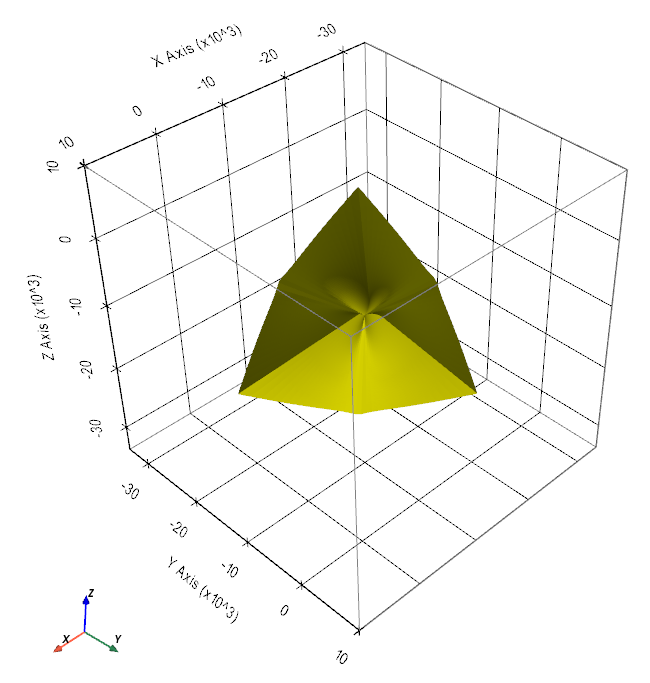
\includegraphics[width=0.7\textwidth]{Figs/mohr_coulomb/MC_sheng_octahedral.png}
  \end{subfigure}
  \begin{subfigure}[t]{0.5\textwidth}
    \centering
    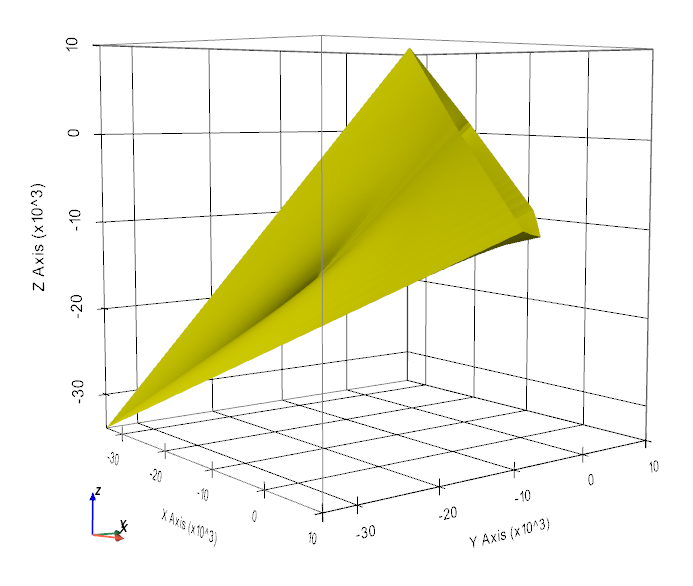
\includegraphics[width=0.7\textwidth]{Figs/mohr_coulomb/MC_sheng_3D.png}
  \end{subfigure}
  \caption{Profiles of the modified Mohr-Coulomb yield surface.}
  \label{fig:MC_Sheng}
\end{figure}
 
